\chapter{Functionality}
\label{chap:functionality}

%This is our webapps functionality,  (3-6 pages of text – %screen dumps in addition)

%\begin{itemize}
%\item Description of the target users 
%\item Description of key features of the application, including key screenshots 
%\item Assessing functional strengths and weaknesses 
%\item Assessing innovativeness 
%\item Description of the innovation/development process 
%\item Discussion of the process used to innovate, develop, and test functionality
%\end{itemize}
\section{Target users}
\label{sec:targetusers}
The target users for this quiz application is rather wide. Our current implementation focuses on birds where everyone from novices to professionals  can participate and exercise. The amazing thing about the quiz is that it can start supporting a new type of quiz really easy for example having a quiz on mammals. It is really expendable and can be adapted to close to any user demographic within the e-learning area. This can be easily extended to work with for example cars, butterflies or even people. Another example is if you have a lot of names to learn it can be adapted to an image quiz on those people. The possibilities are almost endless. That being said, the main target user group is still birds as this is developed under the banner if BirdID. Testing have been done on people with interest in birds, before this project began and the response have been positive, showing that the target users are interested.



\begin{figure}[h]
  \centering
  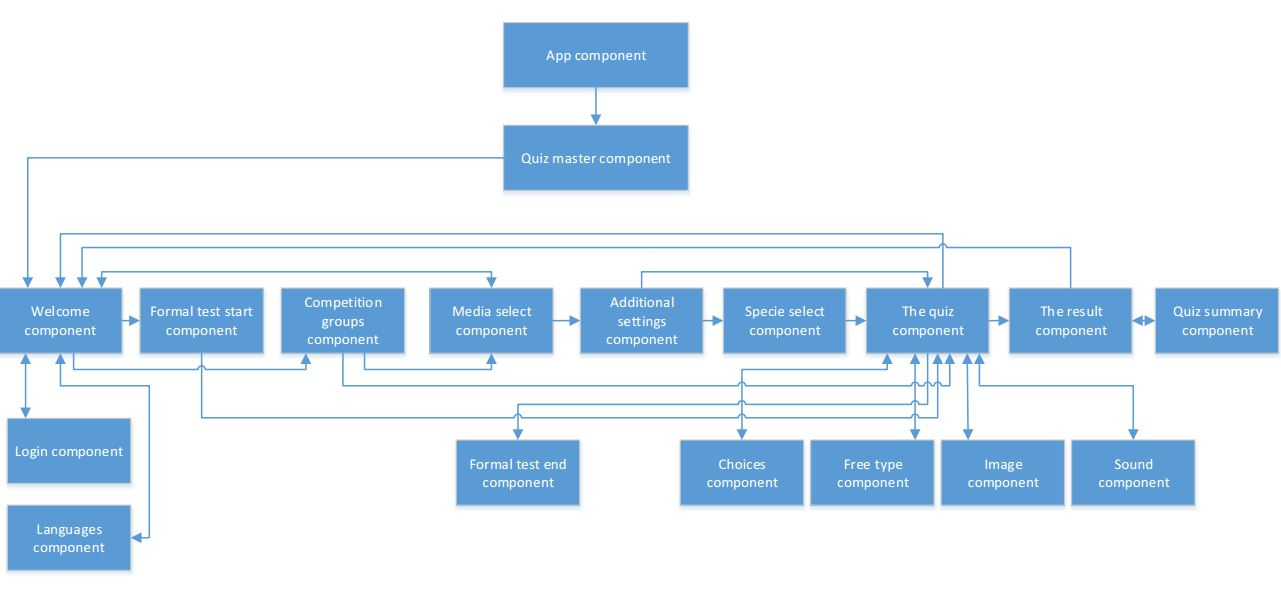
\includegraphics[width=1.0\textwidth]{figures/user_prespective_new.jpg}
  \caption[userPrespective]{The flow of the application }
  \label{fig:userPrespective}
\end{figure}

\begin{figure}[h]
  \centering
  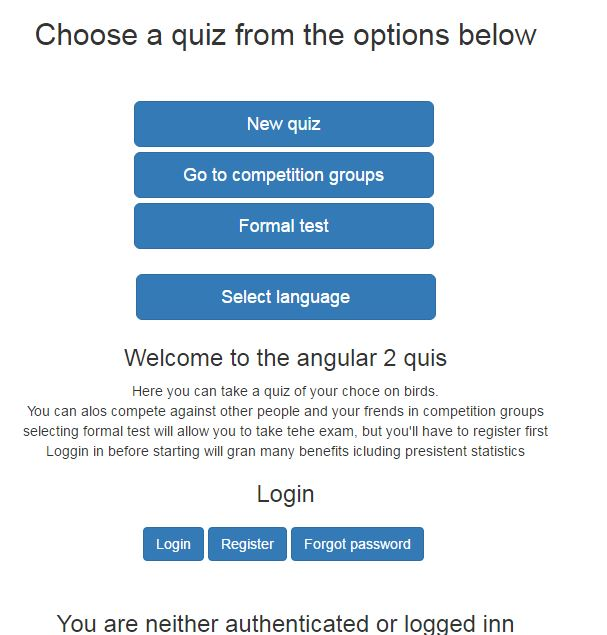
\includegraphics[width=0.8\textwidth]{figures/Welcome.jpg}
  \caption[Welcome]{Welcome}
  \label{fig:Welcome}
\end{figure}

\begin{figure}[h]
  \centering
  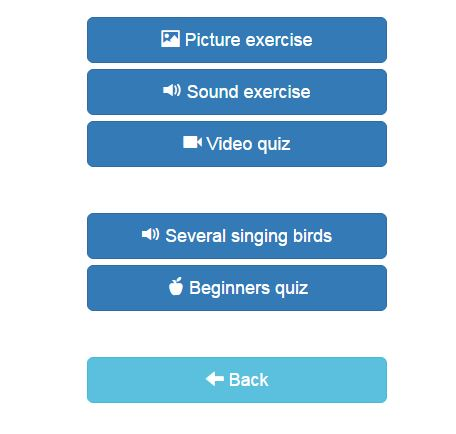
\includegraphics[width=0.6\textwidth]{figures/MediaSelect.JPG}
  \caption[MediaSelect]{Media Select}
  \label{fig:MediaSelect}
\end{figure}
\begin{figure}[h]
  \centering
  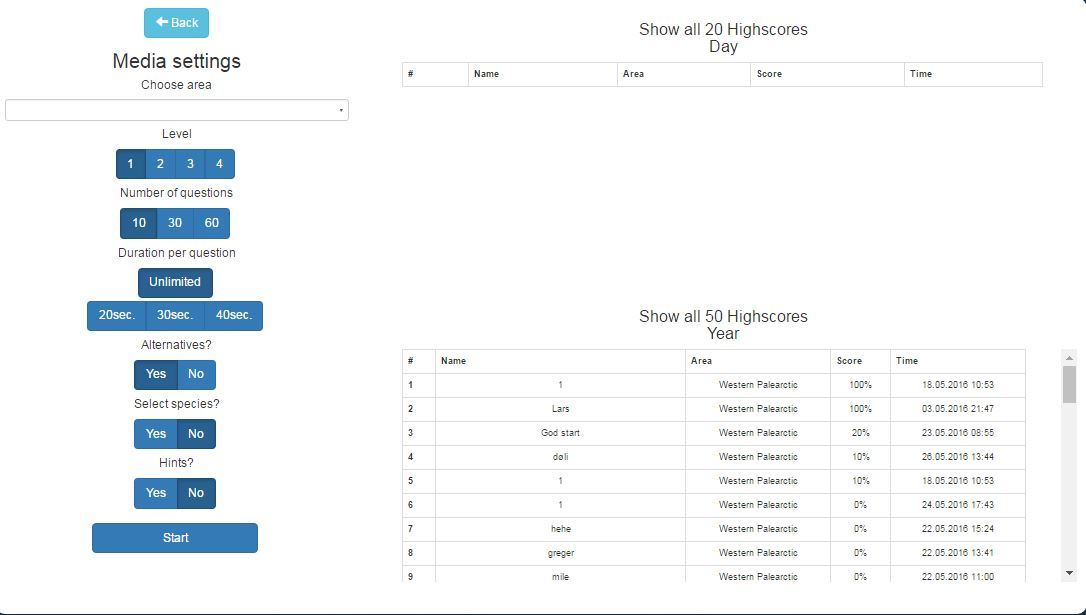
\includegraphics[width=1.0\textwidth]{figures/MediaSettings.JPG}
  \caption[MediaQuizSettings]{Media quiz settings}
  \label{fig:MediaQuizSettings}
\end{figure}

\begin{figure}[h]
  \centering
  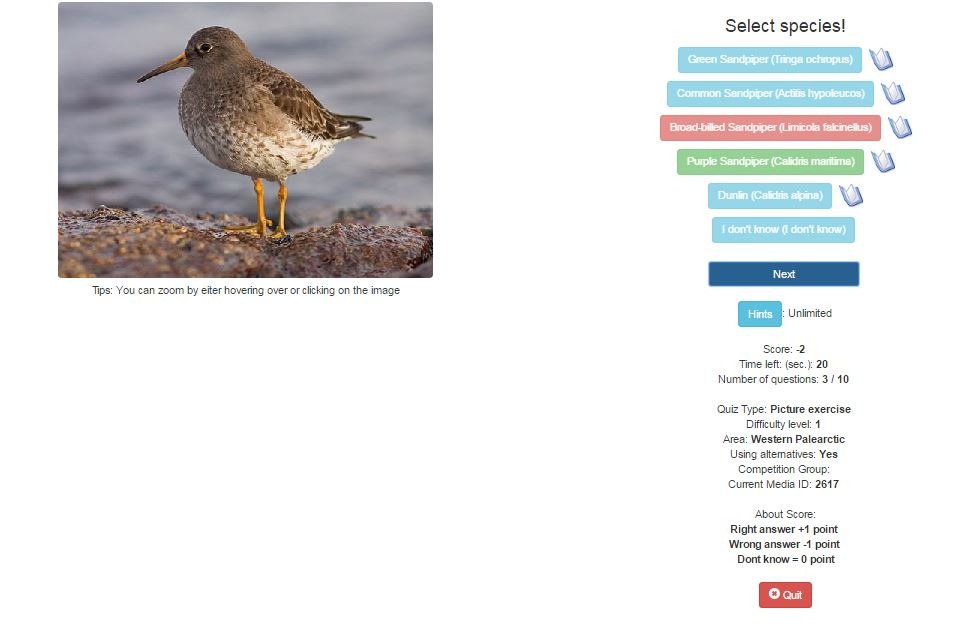
\includegraphics[width=1.0\textwidth]{figures/Quiz.JPG}
  \caption[MediaQuiz]{Media quiz}
  \label{fig:MediaQuiz}
\end{figure}




\begin{figure}[h]
  \centering
  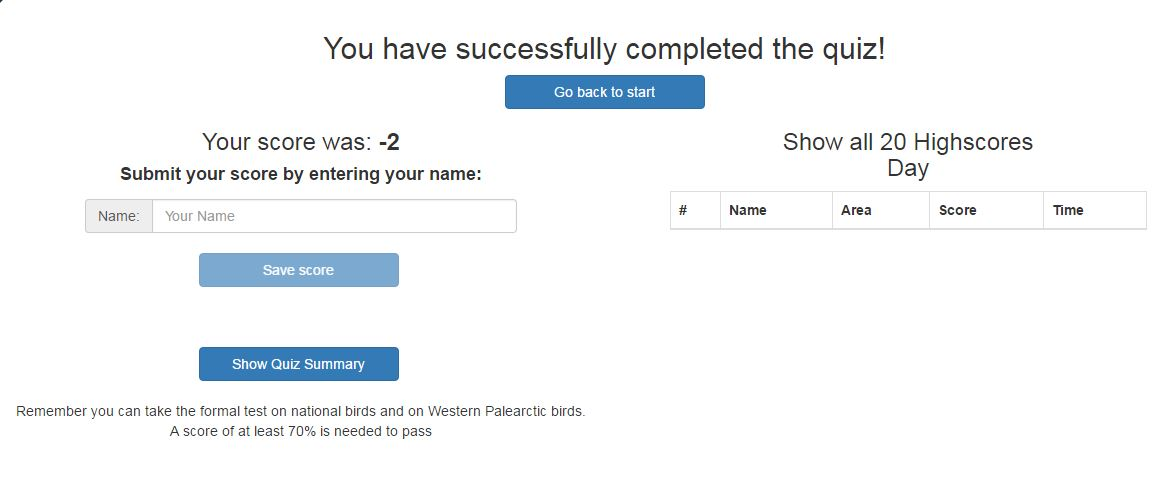
\includegraphics[width=1.0\textwidth]{figures/MediaQuizResults.JPG}
  \caption[MediaQuizResults]{Media quiz results}
  \label{fig:MediaQuizResults}
\end{figure}




\section{Key features}
\label{sec:keyfeatures}
The application has four core quizzes and five core features:
\begin{enumerate}
    \item The quiz
    \begin{itemize}
        \item Image quiz
        \item Sound Quiz
        \item Several Sound Quiz
        \item Beginner Quiz
    \end{itemize}
    \item Competition groups
    \item Formal Test
    \item Changing language
    \item Authentication
    \begin{itemize}
        \item Login
        \item Register 
        \item Forgot /reset password
    \end{itemize}
\end{enumerate}

\break



Image, sound and several sound quizzes are self explanatory types. The users can take quiz where they are presented with images, sound or several sounds playing at the same time. In the several sound quiz since there are multiple birds singing at the same time there is more than one correct answer.


The beginner quiz is a nice way for the user to dive into learning about birds, it has the least difficulty level and it provides a image and a sound from the bird to maximize the users knowledge. 

For all types of quizzes explained above the user can specify additional settings. The users can select a specific area that the quiz will be focused on, the number of questions the user want to answer, limited/unlimited time to answer each question, alternatives or free type meaning that the user want to type the name of the bird or they want to select from predefined choices, the user can select species that are found in the area that they selected previously and in the end they can chose if they want to get hints during the quiz, for the current implementation the user has unlimited hints where each hint is deleting one wrong alternative and gives one letter on each trigger when the user is in the free type quiz. The users can not submit the result if they have selected the hints option, this is to prevent user from cheating the system.


There are two more types of quizzes, competition groups and formal test. Competition groups can hold predefined settings and can be password protected, allowing the users to compete among each other inside the group. If the group does not have predefined settings then the user can select them from the additional settings. \newline
Formal test on the other hand is the official exam that you can take from the Nord University. If the user wants to take the formal test they are advised to get answer 70\% of the questions correct in the normal quiz. Taking a formal test provides a lot of extra security features, but they are handled on server side in order to make it secure. 


\section{Functionality strengths and weaknesses}
\label{sec:functstengwek}
The quiz application contains a lot of functionality and most of it is not really visible or working under the hood for making a smooth experience. The quiz features a lot of customization of settings, allowing the users to tailor the quiz to their needs and therefore offers a lot of replay ability. The questions in the back-end API are in a rather high volume as well, where it has several thousand questions/tasks on the current development server, but an outstanding 25 000 media on the live server. The change of getting the same question/task twice is therefor really low. Each time someone takes the quiz they will get a different quiz than earlier and this might be one of the greatest strengths of the quiz. This is also a major downsides as well since the server return a random list of questions. This makes it really hard to compare your results to the people as they might have gotten slightly easier questions. This does of course even out over several quizzes. This is attempted to be partially solve in the competition groups where the pool of questions is severely limited, but there is still an element of randomness.

The user is able to create and use an account with the quiz. This brings great benefits to the user like tracking persistent statistics and helping the user focus on those species they are having problems with. A lot of the benefits of this is provided on the website, and not in the quiz. However the actual statistic are gathered by the current quiz application and transmitted to the server if the user is logged in. Future iteration in the quiz might have some of this functionality integrated, for example, taking a quiz on your 10 worst species.

Another strength of the application is localisation feature that provides translations (on the live version) for over 20 languages. This will allow user to take the quiz in their local language and will greatly help non Norwegian or English speaking people. Most bird watchers know bird names only in the local language and sometimes in Latin (which are both provided). The website is determining the language automatically but the user can of course change it and it saves it to next time.

One weakness is the lack of user testing currently in the quiz application. We did one guerrilla testing session for digital innovation and got a lot of great feedback, but it was one time thing with a rather limited pool of test people. Further testing need to be done to improve the functionality of the application as most of the features need the user input to become perfect. 


The application offers responsiveness in its design allowing users to use the quiz application on any device they would prefer. We also have made it work with electron, making it work as a native application on all computers. This can be a great benefit for user who want a more native experience and separate the quiz application from the browser. The responsive art translates to the native application as well as making it work with both small and large device sizes. It is developed with Bootstrap and a mobile first approach for having the best functionality and experience across devices.

 
 \section{Assessing innovativeness}
 
The main innovation in this project is the structure of the application, but also the tools used and the frameworks used in the development. Close to every part of the project is using new technologies, all the way from angular 2 to Sass, typescript, bootstrap and gulp. Even the API was upgraded from an old XML based interface to JSON based. The entire project was to innovate on the current flash based quiz in the best way possible. The new quiz was faster to develop, is running better and has a really improved user experience, it goes beyond its predecessor. The content of the actual quiz did not change that much, mostly focusing on a massive change and improvement in regards frameworks used. Innovation was also to be found in the development process where state of the art tools like JIRA and Slack was used. We also prompted to use Planing Poker, where we estimated our tasks in story points, further improving on the groups productivity. This is also the first real team  based development of BirdID leading to improvements of the total output.

The original quiz was made in Flash a long time ago when HTML 5 was just a wet dream by developers. The new quiz is however using all required HTML 5 based technologies for improving the quiz as best as possible. Further improvements of the quiz will probably include the video quiz which will add even more amazing functionality from the HTML 5 catalog.

Another area of innovation is making the entire quiz application mobile friendly, supporting any device from a small mobile phone to an large desktop computer. We made it with great help from both bootstrap and new and amazing CCS3 functionality. More and more user seem to favor mobile and declining to serve that marked would be a horrible choice by us \cite{Mobil51:online}. We are using the CSS media tags for defining important layout changes between devices, allowing for a more tailored experience to the given screen size. We also made all functionality available on all platforms like zooming by hover on desktop and by tapping on mobile. 

Another great area of innovation is how we also made it as a fully working native desktop application using Electron. This will allow any user who want a native like experience like with Slack to have it locally on there own computer. More and more applications are moving to the cloud, but having the option to switch back brings value to some users as it does not technical cost anything extra to keep it compatible with electron native. It loads the website as any browser, just with less sandbox restrictions. It will in any way serve as a great example of how a combination between electron and angular 2 is not just feasible, but maybe even the future of native applications which are not resource intensive, like games.
 


\section {The innovation/development process}
For managing product development Scrum methodology was used. That means that whole development process was divided into 8 sprints. Usually duration of each sprint was 1 week. Our development process includes other features that are typical for Scrum. For instance Scrum daily meetings. In the early stages of the development we slacked a bit on the daily meeting, but as the project progressed and the project got more complex we had daily meetings every day. Most of the time we were working together on the campus, and each team member knew what others were working on. That's why we decided not to have a formal daily meeting every day. We were faced with the problem that team members were working on the same task, which were automatically solved when we got stricter with the daily meetings.
\par
As project management tool we used JIRA. To estimate the difficulty of each issue we used story points in JIRA. Planning poker was used to evaluate each task and to agree within the team the on time that should be spend on each task. In the middle of the project planning poker function became available directly from JIRA. We agreed that using it directly from JIRA was better solution for us. Incorrect estimation of tasks was the reason why our burn-down charts were looking far from perfect. At some point of our development process we started to be more familiar with technologies and some issues were overestimated. Underestimation problems were more common problems at the beginning of the project. And other factor that influence correct estimations was that for different group members it took different time to resolve the issue.
\par
As communication tools we used Skype and Slack. Skype we used mostly for voice conferences when we were not able to meet on campus. We had experience with doing planning poker and sprint planning not only on campus(when all of us are together), but also via Skype. They main advantage of Slack for us was setting up different channels for different topics that related to our project. For project work as a communication tool Slack was more beneficial.
\par
Innovation process started with comparison of Angular 1 and Angular 2 frameworks. We analysed advantages and disadvantages of using both of this frameworks. Nevertheless current version of Angular 2 is still beta and has a lot of bugs, which make work challenging we still decided to use it. 




\section {The process used to innovate, develop, and test functionality}
As we were renewing this quiz platform an bringing it back to life we were looking for a new framework to replace the Flash Technology now used in the previous version of the application. In our perspective this is innovation. The quiz it self is not innovative. There is nothing mind blowing about the features in this quiz that would really make it stand out from other quizzes. That being said, what makes this application innovative is not the quiz it self but rather the way the platform as a whole is build and structured. As of now this is a "bird quiz" but that is only for demo purposes. Because of the flexible structure of the platform it can be easily modified to contain whatever topic wanted. It is also developed in a brand new and cutting edge web application framework, Angular 2\cite{Angular2:online}.

\par
Angular 2 is as mentioned a brand new framework for developing web applications. The reason we went with Angular 2 is first and formal that it has been recognized as a framework with a bright future. The Angular 2 framework is supported by Google and there is, in our experience, a lot of resources put into this new framework. Our first decision was the choice between AngularJS\cite{Angul93:online} and Angular2. Some of the project members had worked with AngularJS before, and their experience was mixed. Because of this the project group wanted to go for the new Angular 2. Even though we went with Angular 2 we were sceptical. Reason being it was still in early beta. Working with a framework in beta can be painful for different reasons. First of all, the framework is still in development and could receive breaking changes at any moment and it almost always contains bugs. This means that breaking changes could break the platform over night and bugs could appear around the next corner. One should never underestimate the frustration coming from bugs. A framework in beta with poor documentation and with little public information on the Internet makes it at times hard to know if you are using the framework wrong or if there is a bug breaking your code. But everything taken into consideration we still went for Angular 2 as it also were recommend by our supervisor as well at it would make our application even more innovative.  

\par
As the project progressed we started looking into testing. Our only problem was that at this time the testing documentation was non-existing. We at this point decided to postpone the testing until the official documentation was released. We later read that the team behind Angular2 were currently working on the testing documentation. Though, it turned out that their documentation was delayed. We discussed if we were going to implement testing at the latest part of the project, but we decided that it had no purpose to implement testing just to have them. As we did not implement tests while developing and rather decided to have a thorough session of both black and white testing.



